\documentclass{article}

\PassOptionsToPackage{numbers,square,sort&compress}{natbib}
\usepackage[preprint]{neurips_2024}
\usepackage[T1]{fontenc}
\usepackage[utf8]{inputenc}
\usepackage{microtype}
\usepackage{amsmath, amssymb}
\usepackage{booktabs}
\usepackage{float}
\usepackage{graphicx}
\usepackage{xcolor}
\usepackage{enumitem}
\usepackage{titlesec}
\usepackage{hyperref}
\usepackage{url}

\hypersetup{
  colorlinks=true,
  linkcolor=blue,
  citecolor=blue,
  urlcolor=blue,
  pdftitle={Inherited Circuits, Specialized Semantics: A Pre-Deployment Method for Detecting Aliasing Vulnerability in Security Fine-Tuned LLMs}
}

\titlespacing*{\section}{0pt}{1.0ex plus 0.2ex minus 0.1ex}{0.45ex}
\titlespacing*{\subsection}{0pt}{0.8ex plus 0.2ex minus 0.1ex}{0.35ex}
\setlength{\textfloatsep}{0.8em plus 0.3em minus 0.2em}
\setlength{\floatsep}{0.7em plus 0.3em minus 0.2em}
\setlength{\intextsep}{0.8em plus 0.3em minus 0.2em}
\setlength{\abovecaptionskip}{0.35em}
\setlength{\belowcaptionskip}{0.2em}
\renewcommand{\topfraction}{0.9}
\renewcommand{\bottomfraction}{0.8}
\renewcommand{\textfraction}{0.07}
\renewcommand{\floatpagefraction}{0.75}
\setcounter{topnumber}{4}
\setcounter{bottomnumber}{3}
\setcounter{totalnumber}{5}

\title{Inherited Circuits, Specialized Semantics: A Pre-Deployment Method for Detecting Aliasing Vulnerability in Security Fine-Tuned LLMs}
\author{%
  Ryan Fetterman \\
  Cisco\\
   \texttt{rfetterm@cisco.com}
}
\date{}

\begin{document}
\raggedbottom

\maketitle
\begin{abstract}
LLMs are increasingly fine-tuned for specific security classification tasks, and the resulting models are typically evaluated on held-out examples from the same distribution as their training data. We show that this evaluation practice misses a class of vulnerability introduced by the fine-tuning itself: a model trained on a corpus where specific command names are strongly correlated with maliciousness can learn to rely on those command names in ways that make it fail silently on alias substitutions — functionality-preserving rewrites that standard test sets do not include. This brittleness is invisible to accuracy metrics yet directly exploitable.

To understand the mechanism, we apply mechanistic interpretability tools to a natural base/fine-tuned model pair — Llama-3.1-8B-Instruct and its cybersecurity fine-tune Foundation-Sec-8B-Instruct — evaluated on a 293-pair matched cohort of malicious and benign PowerShell scripts. Using causal interventions, we localize the classification circuit to a small set of late attention heads (Layer 12) and show this circuit is inherited from Llama rather than created by fine-tuning. Fine-tuning concentrates and semantically specializes this inherited structure, adding strong associations between full-form command names and malicious classification. Those associations improve accuracy on canonical inputs but create alias attack surfaces: in Foundation-Sec, ablating \texttt{Invoke-WebRequest} command-name tokens \emph{increases} malicious confidence (\(+1.13\) mean delta, positive in 73.7\% of scripts), while Llama shows the opposite (\(-1.60\)). A two-tier evasion benchmark confirms the consequence — Foundation-Sec fails consistently on \texttt{iwr} alias substitution while Llama has zero misses on the same variants.

From this analysis we derive a practical pre-deployment detection method. A linear probe fit from base-model activations at the classification boundary (\(r = 0.80\)--\(0.87\) per head) quantifies family-level representation drift after fine-tuning. A complementary indicator-token sign test — comparing how each model’s confidence changes when command-name tokens are ablated — identifies the specific families where the token role has flipped from driver to suppressor. Together these two signals, computed entirely on canonical clean inputs without generating any evasion variants, provide a prioritized red-teaming target list for post-fine-tuning adversarial evaluation.
\end{abstract}

\textbf{Keywords:} security fine-tuning, aliasing vulnerability, pre-deployment testing, large language models, malware detection, PowerShell, causal intervention

\section{Introduction}
Teams fine-tuning LLMs for security classification typically evaluate the resulting model on held-out examples drawn from the same distribution as the training data. This measures accuracy on canonical inputs but does not reveal whether the model has become reliant on specific command-name tokens in ways that make it vulnerable to alias substitution — replacing a full command name with a short equivalent that preserves all malicious behavior. A model that learned to associate \texttt{Invoke-WebRequest} with maliciousness will classify the canonical form correctly, and will appear fine on held-out test data, while silently failing on scripts that use \texttt{iwr} instead. Standard evaluation cannot detect this because it does not test the substitution.

This paper addresses that gap with a pre-deployment detection method. The core insight is that alias vulnerability has a detectable signature in the model's internal representations, observable on canonical clean inputs before any evasion variants are generated. When fine-tuning causes a command-name token to shift from driving malicious classification to suppressing it — because the model has learned to classify that family through surrounding payload context rather than the command name itself — the token has become an alias attack surface. This shift is directly measurable: ablate the command-name tokens from canonical malicious scripts, compare the change in confidence between the base model and the fine-tuned model, and flag families where the sign diverges. A family where the fine-tuned model's confidence increases when command tokens are removed (suppressor role) while the base model's confidence decreases (driver role) is the target for alias red-teaming.

We validate this method on Foundation-Sec-8B-Instruct and its base model, Llama-3.1-8B-Instruct, using a 293-pair matched cohort of PowerShell scripts and a two-tier evasion benchmark. The indicator-token sign test identifies \texttt{Invoke-WebRequest} as the family with the clearest model divergence. The evasion benchmark confirms it: Foundation-Sec fails consistently on \texttt{iwr} alias substitution, while Llama has zero misses on the same variants. The sign test result, computed entirely on canonical inputs, correctly anticipates this outcome before any evasion variant is attempted.

The contributions of this paper are:
\begin{itemize}[leftmargin=1.5em,itemsep=0.15em,topsep=0.15em,parsep=0pt,partopsep=0pt]
  \item A pre-deployment detection method for aliasing vulnerability in security fine-tuned LLMs: a linear probe at the classification boundary flags families with representation drift, and an indicator-token sign test identifies families where command-name tokens shifted from driver to suppressor role — the specific condition that enables alias substitution attacks.
  \item Validation on a Foundation-Sec / Llama model pair: the sign test correctly identifies \texttt{Invoke-WebRequest} as the vulnerable family on canonical inputs, and the evasion benchmark confirms consistent misses on \texttt{iwr} substitution that Llama does not share.
  \item A two-tier syntax-preserving evasion benchmark constructed from matched seed/variant pairs, enabling attribution of failures to specific token transformations.
  \item The finding that prompt-level mitigations trade one vulnerability for another: fixing \texttt{Invoke-WebRequest} alias misses via prompt engineering simultaneously opens new misses on \texttt{Invoke-Expression} obfuscation, motivating pre-deployment testing over post-deployment patching.
  \item Evidence that the classification circuit is inherited from the base model rather than created by fine-tuning, with fine-tuning adding semantic specialization on top of an existing structure — which means the vulnerability profile is set jointly by the base model and the fine-tuning data distribution.
\end{itemize}

\begin{table}[!htbp]
\centering
\small
\setlength{\tabcolsep}{4pt}
\renewcommand{\arraystretch}{0.95}
\caption{Claim ladder for the current study. This table separates what is treated as discovery context from what is treated as the main validated claim.}
\label{tab:claim-ladder}
\begin{tabular}{@{}p{0.11\linewidth}p{0.4\linewidth}p{0.47\linewidth}@{}}
\toprule
Claim level & Main statement & Role in this draft \\
\midrule
Discovery & Early Layer 0 detector family, especially \texttt{L0H11} and \texttt{L0H9} & Initial localization result motivating the narrower validated route, but not final evidence by itself \\
Validation & \texttt{L0H11 $\rightarrow$ L12H15/L12H5/L12H4} & Cleanest minimal direct branch on the 293-pair cohort \\
Validation & \texttt{L12H15/L12H5/L12H4/L12H28} & Stronger late-stage bundle on the 293-pair cohort \\
Refinement & \texttt{L12H2} helps some grouped ablations but weakens the main patching comparison & Auxiliary family-sensitive helper rather than part of the stable sufficiency core \\
Comparison & Llama shares \texttt{L0H11} and Layer 12 but shifts late dominance toward \texttt{L12H28} & Evidence that fine-tuning reshapes an inherited circuit rather than creating the structural route \\
Evasion & \texttt{invoke\_webrequest\_alias} and \texttt{invoke\_expression\_format\_string} preserve late malicious evidence but reverse its downstream effect & Mechanistic reading of the current benchmark failures; supports signal reversal rather than deletion \\
\bottomrule
\end{tabular}
\end{table}

\section{Prior Work}
A body of research has established that transformer-based language models can often be understood in terms of small, identifiable internal components — attention heads and feed-forward layers — that causally drive specific behaviors \citep{cammarata2020thread,elhage2021mathematical}. Studies have shown these components can be identified through causal interventions: selectively disabling or substituting internal activations and measuring how the model's output changes \citep{wang2023interpretability,conmy2023automated}. More recent work has extended these tools toward automated discovery and toward understanding how fine-tuning reshapes these internal structures \citep{ameisen2025attributiongraphs,wang2025finetuningcircuits}. A consistent finding is that fine-tuning tends to modify how existing components are weighted and used rather than creating entirely new structures from scratch — which is directly relevant to interpreting our Foundation-Sec results.

The model lineage matters for interpretation. Foundation-Sec-8B was built from the Llama 3.1 8B base architecture through continued pretraining on a curated cybersecurity corpus \citep{kassianik2025foundationsecbase}. Foundation-Sec-8B-Instruct extends this with instruction tuning for chat-style security use \citep{weerawardhena2025foundationsecinstruct}. The model was previously evaluated favorably in PowerShell classification, with a reported \(+16\%\) precision gain over the baseline in a threat-hunting workflow \citep{fetterman2025foundationsecpowershell}. Because Foundation-Sec and Llama share the same underlying architecture, any differences in their internal classification behavior can be attributed to fine-tuning rather than to architectural changes — making this a clean comparison for isolating what security fine-tuning adds or changes.

The evasion side of this paper connects to a broader pattern in security research: detectors that perform well on canonical inputs can fail under functionality-preserving rewrites that fall outside the training distribution \citep{lucas2023adversarial,mukherjee2023evading}. The specific concern here — that LLM-based classifiers may rely on brittle surface indicators — is the same concern, applied to a model whose internal mechanism can now be examined directly.

\section{Background}
Readers familiar with transformer internals can skip this section. For those new to the concepts, the following definitions are sufficient to follow the paper.

A transformer processes text by passing it through a sequence of \emph{layers}. Each layer contains two types of components: \emph{attention heads}, which look back at earlier parts of the input and pull in relevant information, and \emph{MLP blocks} (feed-forward sublayers), which apply learned transformations to the current state. All components write their outputs into a shared running representation called the \emph{residual stream}, which accumulates information across layers and ultimately determines the model's output. The notation \texttt{L12H15} means Layer 12, Attention Head 15. \texttt{resid\_pre13} refers to the state of the residual stream immediately before Layer 13 — the point we use as the classification boundary in this study.

We use the term \emph{circuit} to mean a small subset of model components — specific attention heads and MLP blocks — whose outputs causally determine the model's classification decision for a given input type. Identifying a circuit means showing that these components are both necessary (removing them weakens the decision) and sufficient (copying their activations from a malicious example into a benign context recreates the malicious classification). A \emph{route} is one specific pathway through that circuit, and a \emph{late-stage bundle} is the group of late-layer heads that carry the strongest classification signal near the output.

Two intervention techniques drive the analysis. \emph{Path patching} tests sufficiency: copy the internal activations of a candidate route from a malicious script into the same positions in a benign script, and measure how much the classification score shifts toward malicious. \emph{Head ablation} tests necessity: disable a candidate group and measure how much the malicious classification weakens. When we say a route is \emph{validated}, we mean it passes both tests on the 293-pair matched cohort. When we say \emph{signal inversion}, we mean the model still internally generates evidence of maliciousness, but a later component reverses how that evidence affects the final output.

\section{Problem Setting}
The task is binary malicious-code classification for PowerShell scripts. The key mechanistic difficulty is that many suspicious strings are not uniquely malicious: benign administrative scripts can contain tokens such as \texttt{IEX}, \texttt{FromBase64String}, \texttt{DownloadString}, \texttt{Invoke-WebRequest}, or \texttt{-EncodedCommand}. We therefore use matched benign and malicious examples sharing suspicious indicators, so that the interpretability problem is not trivially solved by superficial token presence alone.

\section{Dataset and Evaluation Cohorts}
\subsection{Source Dataset}
The source corpus contains 2{,}556 labeled PowerShell scripts, derived from prior work\citep{FANG202130}. The class balance after filtering is approximately even. A substantial long tail of long scripts motivated  a 12,000-character pre-processing cap when building the analysis manifests and construction of the matched cohorts, so benign and malicious scripts were paired and selected under explicit length control rather than letting the very longest scripts dominate the mechanistic runs. The main evidentiary basis for this draft is a 293-pair within-family matched cohort drawn from 456 unique scripts across the seven indicator families, in which benign and malicious scripts share suspicious indicators while remaining length-controlled enough for the intervention pipeline. This cohort was filtered from 380 candidate pairs by requiring both members of each pair to be correctly classified at baseline. 

\section{Methods}
\subsection{Discovery}
The goal of the discovery phase is to identify a small number of candidate components that repeatedly carry malicious-versus-benign evidence before we run the stronger causal tests below. We first examine which attention heads consistently focus on suspicious command spans, URLs, or execution sites across matched script pairs. We then run coarse ablations — disabling individual heads or entire layer bands — to ask whether removing a candidate weakens the malicious classification enough to justify studying it further \citep{cammarata2020thread,elhage2021mathematical,conmy2023automated,ameisen2025attributiongraphs}.

Two discovery techniques are especially important. First, we define a \emph{malicious direction} in the model's internal representation — a vector pointing from how the model represents benign scripts toward how it represents malicious ones — and test whether specific internal sites are pushing the model along that direction. This distinguishes components that are genuinely carrying classification-relevant evidence from those that are merely active. Second, we decompose the contribution at each site into individual head outputs, which lets us identify a small set of dominant heads rather than treating an entire layer as a black box. These analyses narrow the search space so that the final causal claim can be stated precisely rather than vaguely attributed to ``early'' or ``late'' layers.

\subsection{Validation}
The final claim is based on grouped interventions on the 293-pair cohort:
\begin{itemize}[leftmargin=1.5em,itemsep=0.2em,topsep=0pt,parsep=0pt,partopsep=0pt]
  \item \textbf{Grouped path patching} is used primarily as a sufficiency test.
  \item \textbf{Grouped head ablation} is used primarily as a necessity test.
\end{itemize}

In simple terms, a \emph{sufficiency} test asks whether a candidate route is enough to recreate the relevant behavior when its activations are patched in from a malicious example. A \emph{necessity} test asks whether the behavior weakens when that route is removed or disabled. These are related but not identical questions: a route can be sufficient without being strictly necessary if the model has backup pathways, and it can be necessary in a narrow setting without being the cleanest transportable route for patching.

Throughout the paper, \emph{mean intervention effect} refers to the average shift produced by an intervention on the model's malicious-versus-benign decision score, measured as the post-intervention score minus the original score. A more negative mean effect therefore indicates that the intervention weakens the malicious judgment; for patching and ablation experiments that remove or corrupt the route, larger negative values indicate stronger causal dependence on the removed route. \emph{Flip rate} reports how often that intervention is strong enough to change the model's final predicted label.

\subsection{Evasion}
We evaluate syntax-preserving obfuscation techniques and then, for the strongest misses, compare each original malicious script with its rewritten variant using the same circuit probes. Candidate variants are generated only from malicious seed scripts that the model initially classifies correctly, so the evasion benchmark measures failures relative to seeds that already pass the baseline classifier. Throughout this section, \texttt{evasion} means behavioral evasion of classification, that is, a malicious variant that the model now predicts benign. The central mechanistic question is whether successful evasion removes the validated malicious-evidence route or instead preserves that route while later computation changes how that evidence is used. In the best-localized current case, this change appears at the Layer 13 boundary: feed-forward computation before that boundary introduces a competing signal that reverses the effect of the surviving late-stage bundle.

The implemented benchmark is two-tiered. \texttt{direct\_v1} relies on alias substitution, call-operator indirection, token splitting, and literal or method-name reconstruction. \texttt{reconstructive\_v2} stresses the classifier with character-level and command-reconstruction patterns that are often seen in obfuscated PowerShell, including backticks, format strings, ASCII or Base64 recovery, invisible Unicode normalization, and alternate quoting or subexpressions. The benchmark schema defines five broad evasion families; this draft instantiates the \texttt{keyword\_hiding}, \texttt{string\_construction}, and \texttt{execution\_indirection} families.

\begin{table}[!htbp]
\centering
\caption{Two-tier evasion benchmark structure. The \texttt{direct\_v1} tier applies direct syntax-preserving rewrites to visible command, token, and method forms, while \texttt{reconstructive\_v2} uses composed expressions that reconstruct suspicious commands or strings at runtime. Variants are accepted only after parse and invariant checks for valid PowerShell syntax.}
\label{tab:evasion-methods}
\begin{tabular}{p{0.03\linewidth}p{0.18\linewidth}p{0.44\linewidth}p{0.3\linewidth}}
\toprule
Tier & Family & Representative rewrite & Current role \\
\midrule
\texttt{v1}& \texttt{keyword hiding}& \texttt{Invoke-WebRequest ...} $\rightarrow$ \texttt{iwr ...} & Direct rewrite of visible command tokens.\\
\texttt{v1}& \texttt{execution indirection}& \texttt{iex \$x} $\rightarrow$ \texttt{\& ([scriptblock]::Create(\$x))} & Preserve execution while replacing direct invocation with call-operator indirection. \\
\texttt{v1}& \texttt{string construction}& \texttt{DownloadString(...)} $\rightarrow$ \texttt{PSObject.Methods ['Download'+'String'].Invoke(...)}& Direct method-name reconstruction without changing payload behavior.\\
\texttt{v2}& \texttt{keyword hiding}& \texttt{Invoke-Expression} $\rightarrow$ \texttt{\&(('{0}{1}' -f 'Invoke-','Expression'))} & Runtime command reconstruction through format strings or related expressions.\\
\texttt{v2}& \texttt{string construction}& \texttt{Invoke-WebRequest} $\rightarrow$ Base64/ASCII, subexpression, or zero-width-normalized reconstruction & Runtime recovery of suspicious strings or command forms.\\
\bottomrule
\end{tabular}
\end{table}

The implemented benchmark pipeline is more specific than a generic ``obfuscation sweep.'' It first builds a malicious seed manifest restricted to baseline-correct malicious scripts. It then applies only a fixed set of allowed rewrites from the requested preset (\texttt{direct\_v1} or \texttt{reconstructive\_v2}), and each rewrite is used only on scripts where it makes sense. For example, a rewrite that hides \texttt{Invoke-WebRequest} is only applied to seeds that actually contain that command, and a rewrite intended for cross-runtime PowerShell is only used when the target script fits that runtime setting. Each generated variant is then reviewed with static parsing, using the PowerShell parser when the required runtime is available and a \texttt{tree-sitter} fallback otherwise, together with explicit invariant checks to ensure underlying behavior is not changed. The current invariant checks require preservation of URL sets, executable or path-like literals, and \texttt{-EncodedCommand} equivalence where relevant, and they also enforce technique-specific argument-preservation checks such as preserved request arguments or preserved process-launch arguments. The malicious seed / variant pairing is what makes the mechanistic experiments interpretable, we measure the same circuit on the same script content under two conditions (literal token present vs. absent) and attribute any difference in the residual stream directly to the token transformation.

\section{Evaluation \& Results}
\subsection{Results at a Glance}
\begin{itemize}[leftmargin=1.5em,itemsep=0.2em,topsep=0pt,parsep=0pt,partopsep=0pt]
  \item \textbf{Fine-tuning is associated with evasion brittleness absent from the base-model comparison:} Foundation-Sec produces \(6/44\) misses on direct alias substitution and \(4/46\) misses on command reconstruction. Llama has \(0/44\) and \(0/46\) misses on the same variants under the same prompt framing. These failures are specific to the fine-tuned model in this controlled model-pair comparison.
  \item \textbf{Brittleness is family-specific, not uniform:} Failures concentrate in \texttt{Invoke-WebRequest} alias substitution (\(4/4\) misses) and \texttt{Invoke-Expression} format-string reconstruction (\(4/4\) misses). Other tested command families are robust under the accepted variants in the implemented benchmark, but the strongest positive slices are small and should be expanded before treating the rates as population estimates.
  \item \textbf{Sign inversion predicts the vulnerable family at the right granularity:} Ablating \texttt{Invoke-WebRequest} tokens from Foundation-Sec \emph{increases} malicious confidence (\(+1.13\) mean delta; positive in 73.7\% of scripts); the same ablation \emph{reduces} Llama's confidence (\(-1.60\)). This family-level sign flip — observable on canonical inputs without generating any evasion variants — identifies the family that produces consistent misses in the current benchmark and should be treated as the primary pre-deployment red-teaming signal.
  \item \textbf{Prompt-level mitigations trade one weakness for another:} Instructing Foundation-Sec to classify based on overall purpose rather than individual constructs fixes the \texttt{Invoke-WebRequest} misses but simultaneously opens new misses on \texttt{Invoke-Expression} obfuscation. The semantic weighting introduced by fine-tuning is distributed across families and cannot be patched in one place without opening another.
  \item \textbf{The classification circuit is inherited from Llama, not created by fine-tuning:} Causal interventions on 293 matched script pairs confirm that Foundation-Sec relies on a small late-stage attention bundle (Layer 12) that Llama also uses. Fine-tuning concentrated and semantically specialized this existing mechanism; it did not invent it. This matters because the circuit's vulnerability profile appears to reflect both the base model's structure and semantic weighting introduced during fine-tuning.
  \item \textbf{Activation-space monitoring is practical and cheap at family level:} A linear probe from base-model activations at the circuit boundary predicts each head's contribution at \(r = 0.80\)--\(0.87\). Cross-model transfer to Foundation-Sec ablation dependence reaches \(r = 0.41\), making per-script prioritization noisy but supporting family-level red-teaming when averaged across canonical examples.
\end{itemize}

\begin{figure}[!htbp]
\centering
\includegraphics[width=0.92\linewidth]{artifacts/foundation_sec/figure_layer_head_locator.png}
\caption{Layer-head locator for the validated Foundation-Sec route. The visual separates the validated \texttt{L0H11} upstream entry, the minimal late route \texttt{L12H15/L12H5/L12H4}, the \texttt{L12H28} sufficiency add-on, and the auxiliary \texttt{L12H2} helper.}
\label{fig:mechanistic-summary}
\end{figure}

\subsection{Circuit Results}
\subsubsection{Validated Late Route}
On the 293-pair cohort, causal patching supports a minimal direct branch:
\[
\texttt{L0H11} \rightarrow \texttt{L12H15/L12H5/L12H4}
\]
The mean patching effect is approximately \(-3.614\), which means that the intervention reduces the model's average malicious-versus-benign decision margin from about \(4.71\) to about \(1.10\). In other words, it removes roughly \(77\%\) of the average malicious decision margin and flips the final prediction on \(87/293\) pairs (\(0.297\)).

The stronger late-stage bundle is:
\[
\texttt{L12H15/L12H5/L12H4/L12H28}
\]
Its mean patching effect is approximately \(-3.824\), which reduces the same average malicious-versus-benign decision margin from about \(4.71\) to about \(0.89\). In other words, it removes roughly \(81\%\) of the average malicious decision margin and also flips the final prediction on \(87/293\) pairs (\(0.297\)).

The role of \texttt{L12H2} is more nuanced. Removing \texttt{H2} improves the main path-patching result, while the full top-five bundle remains slightly stronger under grouped ablation. Our current interpretation is therefore that \texttt{L12H2} is an auxiliary family-sensitive helper, not part of the most stable sufficiency core.

\subsubsection{Interpretation of Early and Late Stages}
The results support an early Layer 0 detector family, especially \texttt{L0H11} and \texttt{L0H9}. However, the final validated claim in this draft does not rest on a broad early-head story. Instead, it uses \texttt{L0H11} as the clearest entry point into the validated late route. The stronger late-stage evidence localizes to attention around Layers 12--13 and to feed-forward computation before the Layer 13 boundary that becomes especially important in the successful-evasion setting.

\subsubsection{Family-Level Variation}
The 293-pair cohort also reveals a useful family-level pattern. The best patch route is not identical across all indicator families. The minimal branch is strongest for \texttt{DownloadFile}, the fuller top-five late bundle is strongest for \texttt{DownloadString} and \texttt{IEX}, and the \texttt{H2}-free carrier (late Layer-12 head bundle with L12H2 removed) is strongest for \texttt{-EncodedCommand}, \texttt{Invoke-Expression}, and \texttt{Invoke-WebRequest}. This pattern supports the current interpretation that \texttt{H2} is not part of the most stable sufficiency core. One caveat: the \texttt{-EncodedCommand} family (7 pairs) shows zero flip rate under all patching variants, indicating that the circuit claim is weakest for this family and that it warrants a cautionary note; the other six families show consistent negative mean deltas across all route variants.

At the same time, grouped ablation suggests that \texttt{H2} still contributes a necessity signal across most families: the top-5 bundle (mean \(\Delta = -2.174\)) is stronger than the H2-free carrier (mean \(\Delta = -1.893\)), confirming \texttt{H2} as an auxiliary helper that matters for necessity even while it weakens patching sufficiency. The family-level picture therefore reinforces the write-up distinction between a stable late-stage bundle and a narrower auxiliary helper.

\begin{table}[!htbp]
\centering
\caption{Family-by-family patching results across the four main late-route variants on the 293-pair cohort. Each route cell reports \texttt{mean $\Delta$ / flip rate}, where a more negative \texttt{mean $\Delta$} indicates a stronger weakening of the malicious judgment under the intervention and therefore stronger dependence on the intervened route. Route abbreviations are: Minimal = \texttt{L0H11 $\rightarrow$ L12H15/L12H5/L12H4}, Top-5 = \texttt{L12H15/L12H5/L12H4/L12H2/L12H28}, H2-free = \texttt{L12H15/L12H5/L12H4/L12H28}, and H28-free = \texttt{L12H15/L12H5/L12H4/L12H2}.}
\label{tab:family-results}
\resizebox{\linewidth}{!}{%
\begin{tabular}{lccccc}
\toprule
Family & Pairs & Minimal & Top-5 & H2-free & H28-free \\
\midrule
\texttt{-EncodedCommand} & 7  & \texttt{-1.41 / 0.00} & \texttt{-0.99 / 0.00} & \texttt{-1.27 / 0.00} & \texttt{-1.11 / 0.00} \\
\texttt{DownloadFile}    & 146 & \texttt{-4.84 / 0.20} & \texttt{-5.07 / 0.15} & \texttt{-5.05 / 0.16} & \texttt{-4.41 / 0.07} \\
\texttt{DownloadString}  & 43  & \texttt{-3.77 / 0.44} & \texttt{-4.05 / 0.44} & \texttt{-4.12 / 0.51} & \texttt{-3.56 / 0.30} \\
\texttt{FromBase64String}& 35  & \texttt{-1.19 / 0.37} & \texttt{-1.26 / 0.34} & \texttt{-1.29 / 0.34} & \texttt{-1.09 / 0.34} \\
\texttt{IEX}             & 25  & \texttt{-3.03 / 0.32} & \texttt{-3.44 / 0.32} & \texttt{-3.48 / 0.44} & \texttt{-2.83 / 0.16} \\
\texttt{Invoke-Expression}& 18 & \texttt{-1.46 / 0.50} & \texttt{-1.61 / 0.50} & \texttt{-1.66 / 0.56} & \texttt{-1.34 / 0.44} \\
\texttt{Invoke-WebRequest}& 19 & \texttt{-1.92 / 0.47} & \texttt{-1.88 / 0.42} & \texttt{-1.86 / 0.47} & \texttt{-1.76 / 0.42} \\
\bottomrule
\end{tabular}
}
\end{table}

\begin{figure}[!htbp]
\centering
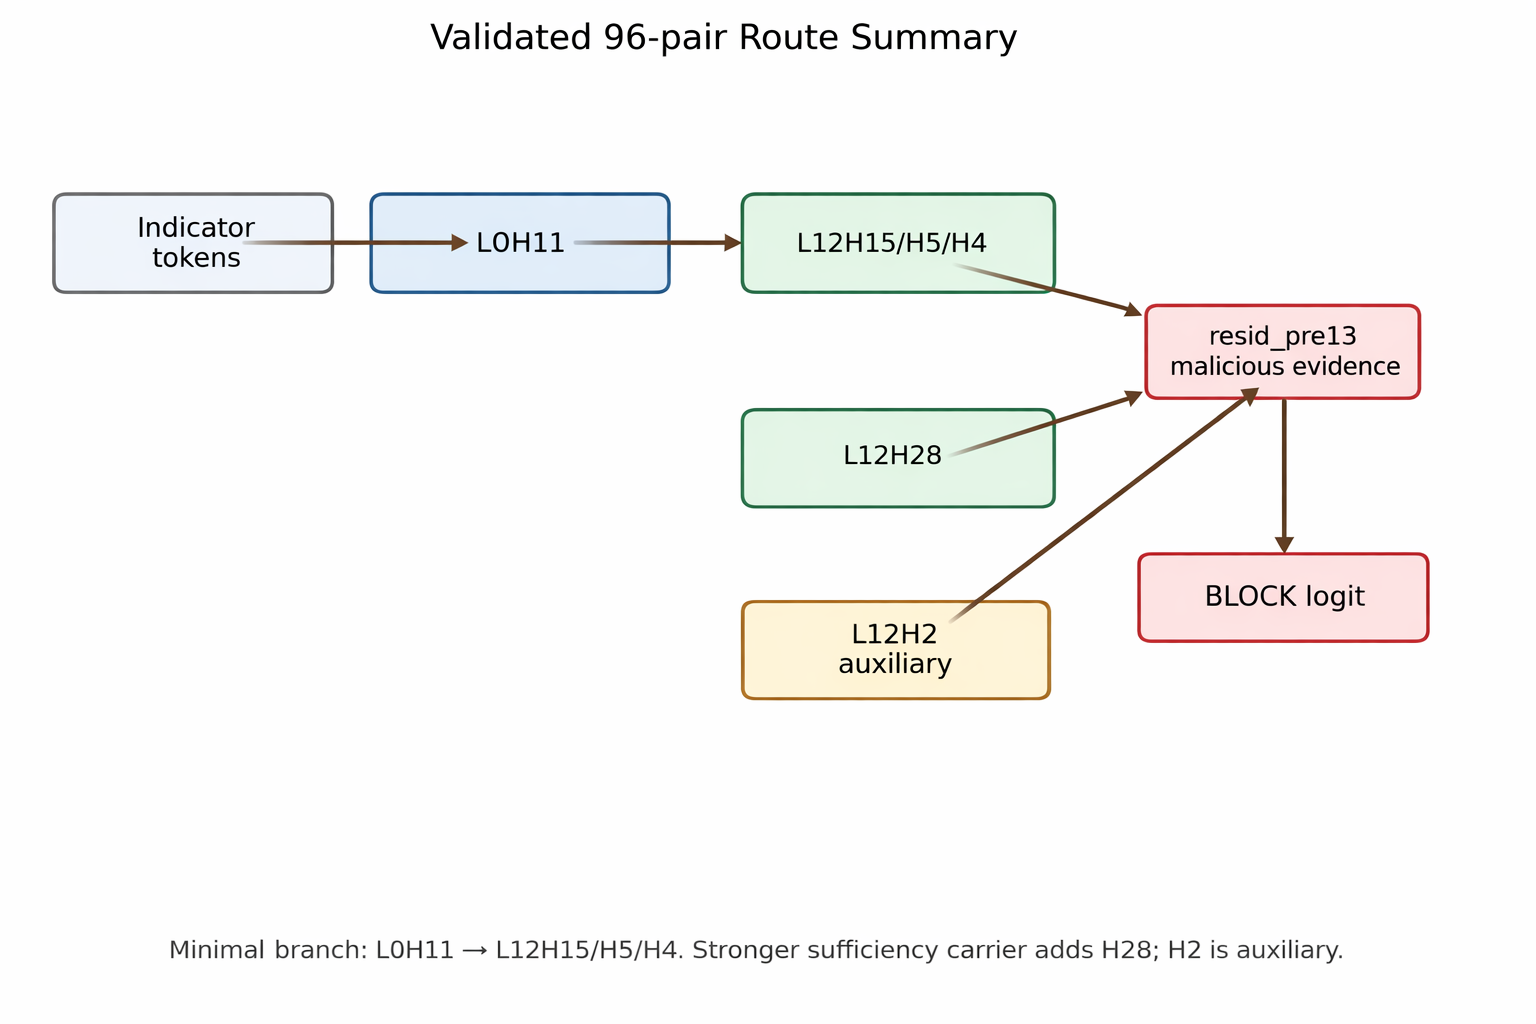
\includegraphics[width=0.92\linewidth]{artifacts/foundation_sec/figure_validated_route.png}
\caption{Conceptual summary of the current validated route. The cleanest minimal branch runs from \texttt{L0H11} into \texttt{L12H15/L12H5/L12H4}, while adding \texttt{L12H28} gives the stronger late-stage bundle. \texttt{L12H2} is shown separately because the current evidence supports it as an auxiliary helper rather than as part of the stable core route.}

\label{fig:route-comparison}
\end{figure}

\subsection{Comparative Model Analysis}
Foundation-Sec and Llama-3.1-8B-Instruct share the same 32-layer, 32-head Llama-3.1 architecture, so the comparison can separate structural inheritance from fine-tuning-specific reweighting. The main comparative result is that the same basic circuit skeleton transfers. In Llama, \texttt{L0H11} is again the most recurrent early detector, appearing in \(14/18\) discovery pairs. The strongest late integration layer is again Layer 12, but the dominant head shifts: Foundation-Sec's route is centered on \texttt{L12H15/L12H5/L12H4/L12H28}, while Llama's traced route is centered on \texttt{L12H28/L12H5/L12H4/L12H13}. This is the pattern expected if cybersecurity fine-tuning concentrated and semantically weighted a pre-existing structural circuit rather than creating a new PowerShell circuit from scratch. 

\begin{figure}[!htbp]
\centering
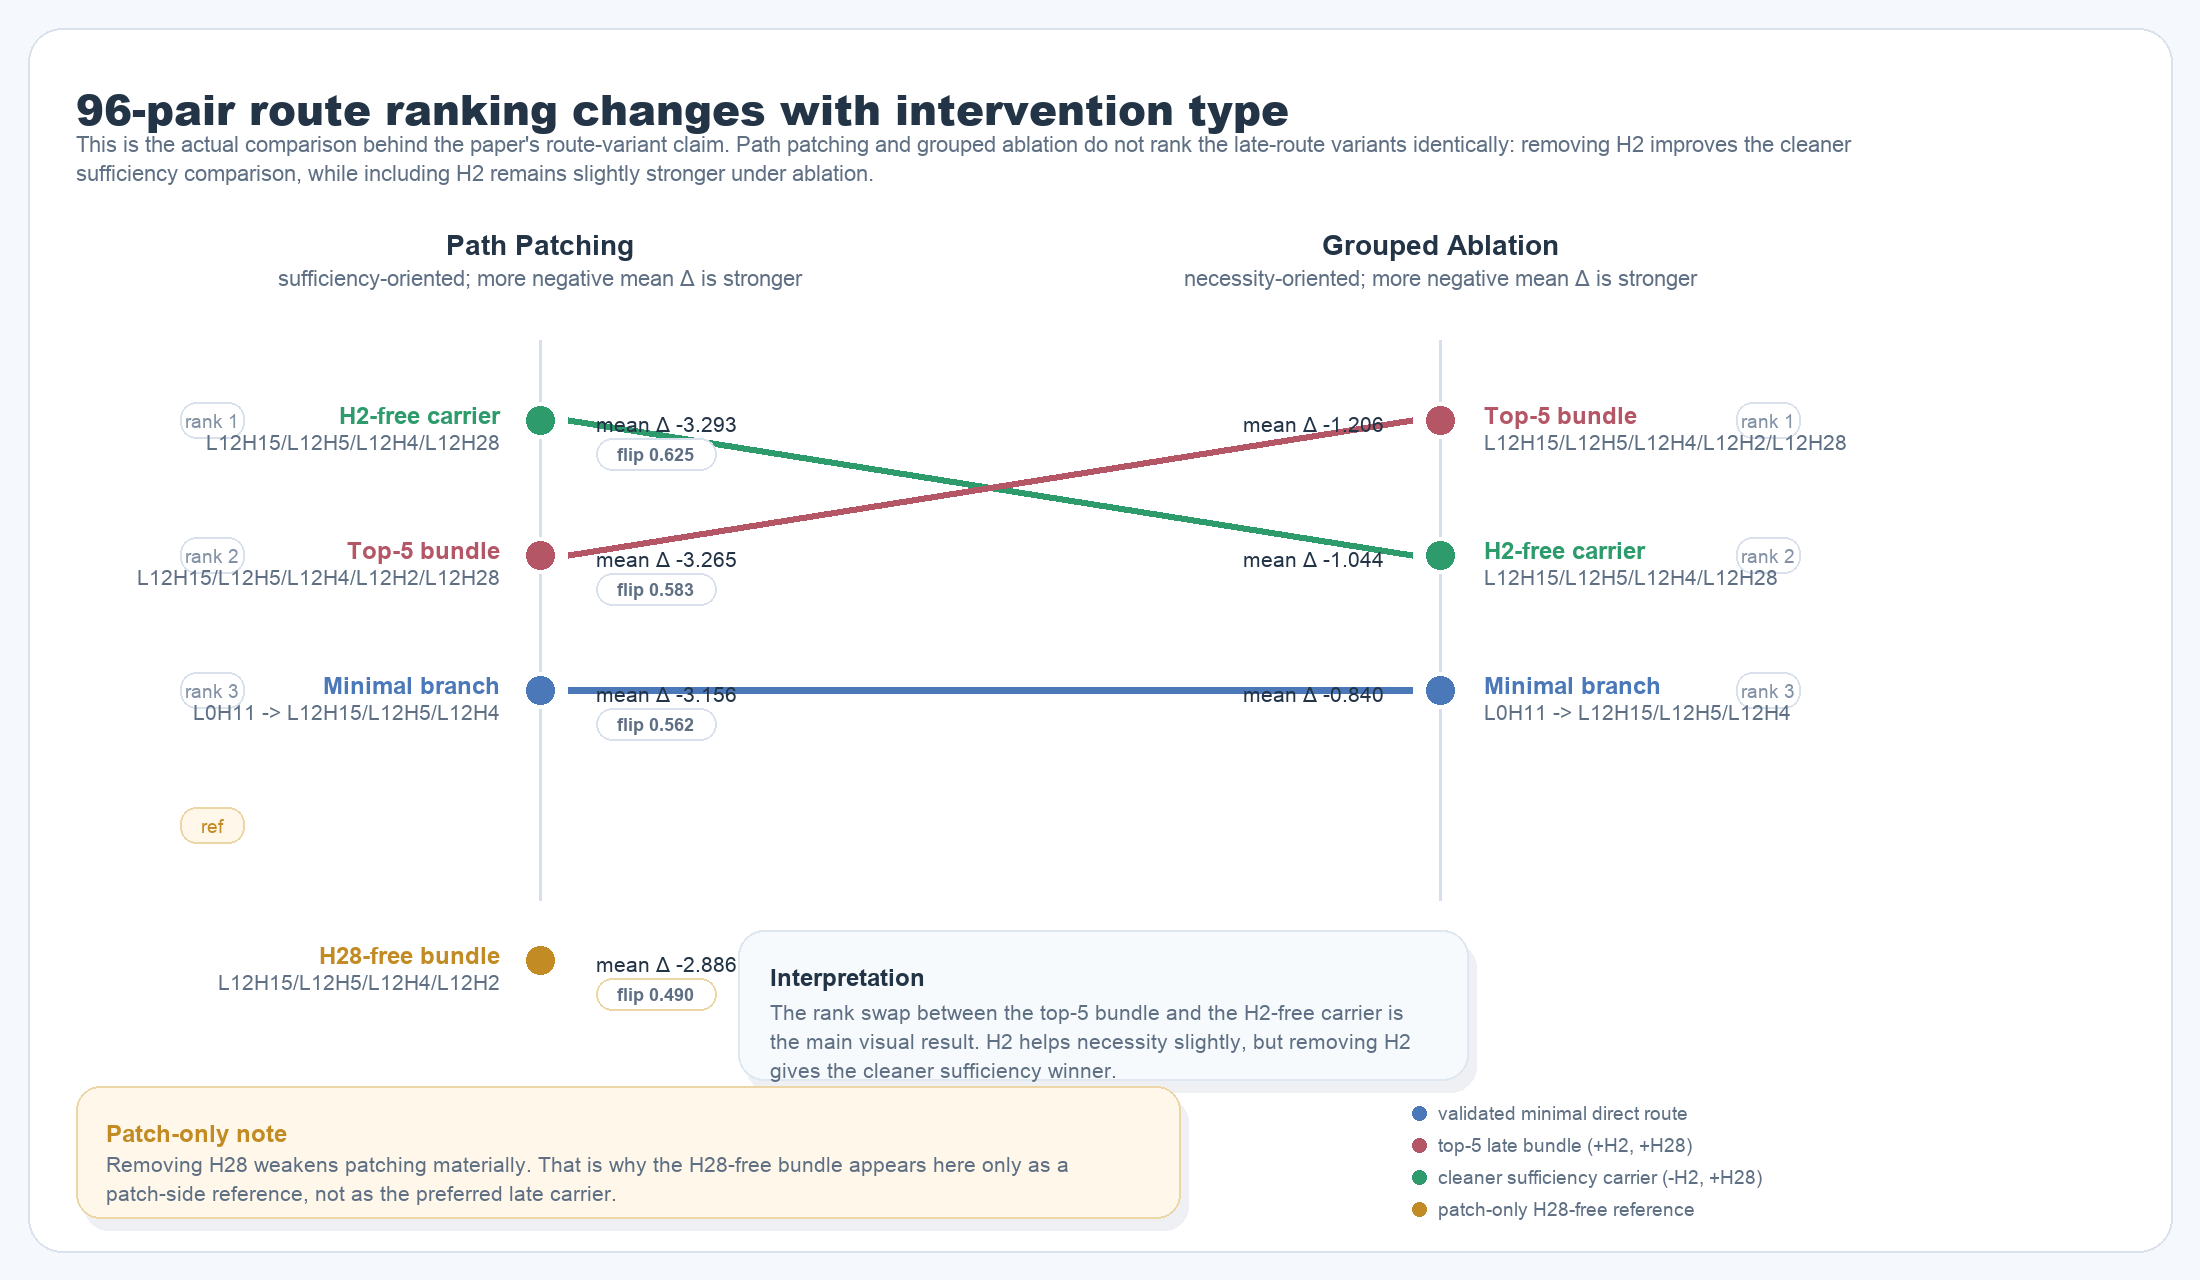
\includegraphics[width=0.92\linewidth]{artifacts/foundation_sec/figure_route_comparison.png}
\caption{Route ranking changes with intervention type in Foundation-Sec. The route variants do not rank identically under path patching and grouped ablation: removing \texttt{L12H2} improves the cleaner sufficiency comparison, while including \texttt{L12H2} remains slightly stronger under ablation.}
\label{fig:shared-skeleton-reweighted-heads}
\end{figure}

\begin{table}[!htbp]
\centering
\small
\caption{Cross-model circuit comparison. Llama uses the same early detector and late writer layer as Foundation-Sec, but its strongest route is more diffuse and shifts late dominance toward \texttt{L12H28}.}
\label{tab:model-comparison}
\resizebox{\linewidth}{!}{%
\begin{tabular}{llll}
\toprule
Metric & Foundation-Sec-8B-Instruct & Llama-3.1-8B-Instruct & Interpretation \\
\midrule
Early detector & \texttt{L0H11} & \texttt{L0H11} & Shared structural entry point \\
Late writer layer & Layer 12 & Layer 12 & Shared late integration stage \\
Top late writer & \texttt{L12H15} & \texttt{L12H28} & Fine-tuning shifts late-head dominance \\
Llama \texttt{L0H11} recurrence & -- & \(14/18\) discovery pairs & Early detector is not Foundation-Sec-specific \\
Minimal route patching & \(24/74\) flips on matched subset & \(-4.865\), \(11/74\) flips & Llama route is sufficient but less compact \\
Stronger route patching & about \(25/74\) flips on matched subset & \(-5.451\), \(18/74\) flips & Same layer, shifted carrier \\
Diffuse bundle patching & about \(25/74\) flips on matched subset & \(-6.158\), \(36/74\) flips & Llama needs a broader head bundle \\
\bottomrule
\end{tabular}
}
\end{table}

This comparison changes the interpretation of the Foundation-Sec results. The cleanest account is not that security training created the \texttt{L0H11}-to-Layer-12 circuit. Instead, fine-tuning appears to concentrate causal weight into a smaller late-head set and add semantic associations between full-form PowerShell command names and the final \texttt{BLOCK} decision. This is consistent with fine-tuning work showing node-level circuit persistence alongside edge and weighting changes \citep{wang2025finetuningcircuits}. On the matched 74-pair adversarial-prompt baseline, that semantic weighting corresponds to a \(4.7\)-percentage-point overall accuracy gain over Llama (\(100\%\) vs.\ \(95.3\%\)), driven entirely by a \(9.5\)-point benign-accuracy improvement (\(100\%\) vs.\ \(90.5\%\)) rather than by improved malicious recall. Notably, fine-tuning does not straightforwardly strengthen the circuit's causal margins: Llama's late carrier mean patching effect is \(-5.45\) versus Foundation-Sec's \(-3.82\) on a comparable route, and Llama's mean base logit diff for malicious examples is \(8.15\) versus Foundation-Sec's \(3.75\). This suggests that fine-tuning concentrates and semantically specialises the circuit without increasing its absolute signal strength, and indeed may attenuate the base model's stronger discriminative representation. The current evidence therefore supports a mechanistic story in which fine-tuning preserves an inherited structural route but adds semantic weighting that can invert the malicious-evidence signal before final readout. That semantic layer is useful for raw-prompt operation, but the evasion benchmark below shows that it also creates a specific attack surface around aliases and command reconstruction.

\subsection{Evasion Results}
Foundation-Sec's results separate cleanly by tier. Because the benchmark is conditioned on baseline-correct malicious seeds, these evasion failures should be read as misses on scripts the model initially handled correctly before rewriting. In \texttt{direct\_v1}, Foundation-Sec stays correct on \(38/44\) accepted variants and the misses are concentrated in two techniques rather than spread broadly across the conservative benchmark. The strongest direct-tier failure remains simple alias substitution in the \texttt{Invoke-WebRequest} family: replacing the full command name with \texttt{iwr} yields misses on all four accepted variants tested. The only other positive result in that tier is narrower. Indirect \texttt{DownloadString} method invocation produces misses in two of six variants, and both of those misses come from \texttt{FromBase64String}-linked seeds rather than from the direct \texttt{DownloadString} seeds themselves.

Foundation-Sec classification accuracy is still strong under the second tier. In \texttt{reconstructive\_v2}, it stays correct on \(42/46\) candidates. All four misses come from one keyword-hiding technique, \texttt{invoke\_expression\_format\_string}. The other reconstructive rewrites---including backtick splitting, Base64 or ASCII reconstruction, subexpression strings, and zero-width normalization for \texttt{-EncodedCommand}---remain negative in the current run. Across both implemented tiers together, Foundation-Sec stays correct on \(80/90\) accepted variants, so the observed weaknesses are specific and technique-concentrated rather than benchmark-wide. Because the positive slices are small, these results should be read as localized counterexamples and red-teaming priorities, not as stable estimates of real-world evasion prevalence.

\begin{table}[!htbp]
\centering
\caption{Foundation-Sec two-tier evasion benchmark status. Most variants satisfy the standard parse and invariant checks from the implemented pipeline.}
\label{tab:evasion-results}
\begin{tabular}{lllll}
\toprule
Tier & Technique or slice & Family & Pairs & Outcome \\
\midrule
\texttt{v1}& \texttt{invoke\_webrequest\_alias} & \texttt{keyword\_hiding} & 4 & $4/4$ misses \\
\texttt{v1}& \texttt{downloadstring\_psobject\_invoke} & \texttt{string\_construction} & 6 & $2/6$ misses \\
\texttt{v1}& all other techniques & mixed & 34 & $0/34$ misses \\
\texttt{v2}& \texttt{invoke\_expression\_format\_string} & \texttt{keyword\_hiding} & 4 & $4/4$ misses \\
\texttt{v2}& all other techniques & mixed & 42 & $0/42$ misses \\
\bottomrule
\end{tabular}
\end{table}

\begin{table}[!htbp]
\centering
\caption{Cross-model evasion comparison under the controlled raw-prompt classifier framing. Llama has no misses on either tier, while Foundation-Sec's misses indicate a prompt-sensitive semantic layer added on top of the inherited structural circuit.}
\label{tab:cross-model-evasion}
\begin{tabular}{llll}
\toprule
Model & Benchmark tier & Variants & Misses \\
\midrule
Llama-3.1-8B-Instruct & \texttt{direct\_v1} & 44 & \(0/44\) \\
Foundation-Sec-8B-Instruct & \texttt{direct\_v1} & 44 & \(6/44\) \\
Llama-3.1-8B-Instruct & \texttt{reconstructive\_v2} & 46 & \(0/46\) \\
Foundation-Sec-8B-Instruct & \texttt{reconstructive\_v2} & 46 & \(4/46\) \\
\bottomrule
\end{tabular}
\end{table}


The Llama result is stable across the evaluated prompt framings: it produces \(0/44\) misses on \texttt{direct\_v1}, and \(0/46\) misses on \texttt{reconstructive\_v2}. Foundation-Sec's failure surface is more prompt-sensitive. Under the raw prompt, Foundation-Sec's misses clustered around techniques that removed specific literal indicator tokens---\texttt{invoke\_webrequest\_alias} (\(4/4\) misses) and \texttt{downloadstring\_psobject\_invoke} (\(2/6\)). Under the adversarial prompt (``classify based on overall purpose, not individual constructs''), \texttt{invoke\_webrequest\_alias} was fully fixed: the model shifted to a more holistic assessment and recovered the malicious intent through other signals. But a new set of misses simultaneously appeared on \texttt{Invoke-Expression} obfuscation variants: telling the model not to weight individual constructs suppressed exactly the command-name associations that had been correctly detecting obfuscated \texttt{Invoke-Expression} patterns. This supports the semantic-layer interpretation: fine-tuning added useful command-name associations, especially around full-form names such as \texttt{Invoke-Expression} and \texttt{Invoke-WebRequest}, but those associations can be bypassed or reshaped by aliases and command reconstruction. The adversarial-prompt comparison also suggests that the inversion itself is Foundation-Sec-specific rather than a generic Llama property: on the same adversarial scripts, Llama's Layer 13 residual stays positive, consistent with the base model lacking the command-name associations introduced by Foundation-Sec's fine-tuning.

\begin{table}[!htbp]
\centering
\caption{Representative side-by-side examples of successful evasion from both benchmark tiers. In \texttt{direct\_v1}, replacing the explicit \texttt{Invoke-WebRequest} token with the alias \texttt{iwr} is sufficient to flip Foundation-Sec's prediction. In \texttt{reconstructive\_v2}, a format-string reconstruction of \texttt{Invoke-Expression} likewise produces a Foundation-Sec miss while preserving the surrounding payload logic.}
\label{tab:evasion-example}
\begin{tabular}{p{0.14\linewidth} p{0.14\linewidth} p{0.64\linewidth}}
\toprule
Tier & Version & Script fragment \\
\midrule
\texttt{v1}& Seed &
\texttt{Invoke-WebRequest -Uri http://stderr.pl/procdump.exe -OutFile c:\textbackslash temp\textbackslash sendme.exe} \\
\texttt{v1}& Variant &
\texttt{iwr -Uri http://stderr.pl/procdump.exe -OutFile c:\textbackslash temp\textbackslash sendme.exe} \\
\midrule
\texttt{v2}& Seed &
\texttt{Invoke-Expression \$(New-Object IO.StreamReader (...)).ReadToEnd();} \\
\texttt{v2}& Variant &
\texttt{\&(('{0}{1}' -f 'Invoke-','Expression')) \$(New-Object IO.StreamReader (...)).ReadToEnd();} \\
\bottomrule
\end{tabular}
\end{table}
The key mechanistic finding on the successful evasion cases is that the internal classification signal does not simply disappear when the alias substitution is applied. Under \texttt{invoke\_webrequest\_alias}, the late-layer attention heads that normally carry malicious evidence still fire on the miss variants — the internal evidence is still there. What changes is how a subsequent feed-forward layer (just before Layer 13) uses that evidence: it reverses the signal, turning what was a push toward malicious into a push toward benign. The evasion is therefore better understood as signal reversal by a later component than as deletion of the detection mechanism. The \texttt{invoke\_expression\_format\_string} misses show the same pattern: the early and late attention components still respond to the malicious content (\(4/4\) variants flip under patching), but their output is overridden downstream. Both cases are consistent with the observation that fine-tuning added command-name semantic associations that interact with the inherited detection circuit in ways that can invert the final output when those command names are absent \citep{lindsey2025biology}.

The current evidence does \emph{not} support a generic statement that direct or reconstructive obfuscation automatically defeats these models. In Foundation-Sec \texttt{direct\_v1}, misses occur only in \texttt{invoke\_webrequest\_alias} and the narrower \texttt{downloadstring\_psobject\_invoke} pattern concentrated in \texttt{FromBase64String}-linked seeds. In Foundation-Sec \texttt{reconstructive\_v2}, misses occur only in \texttt{invoke\_expression\_format\_string}; the other tested backtick, Base64 or ASCII, subexpression, and zero-width-normalization techniques remain robust among the accepted variants in the current run. Llama's controlled raw-prompt results, \(0/44\) misses on \texttt{direct\_v1} and \(0/46\) misses on \texttt{reconstructive\_v2}, show that the same architectural circuit can be less brittle when it remains more diffuse and less tied to Foundation-Sec's full-form command-name semantics.

\begin{figure}[!htbp]
\centering
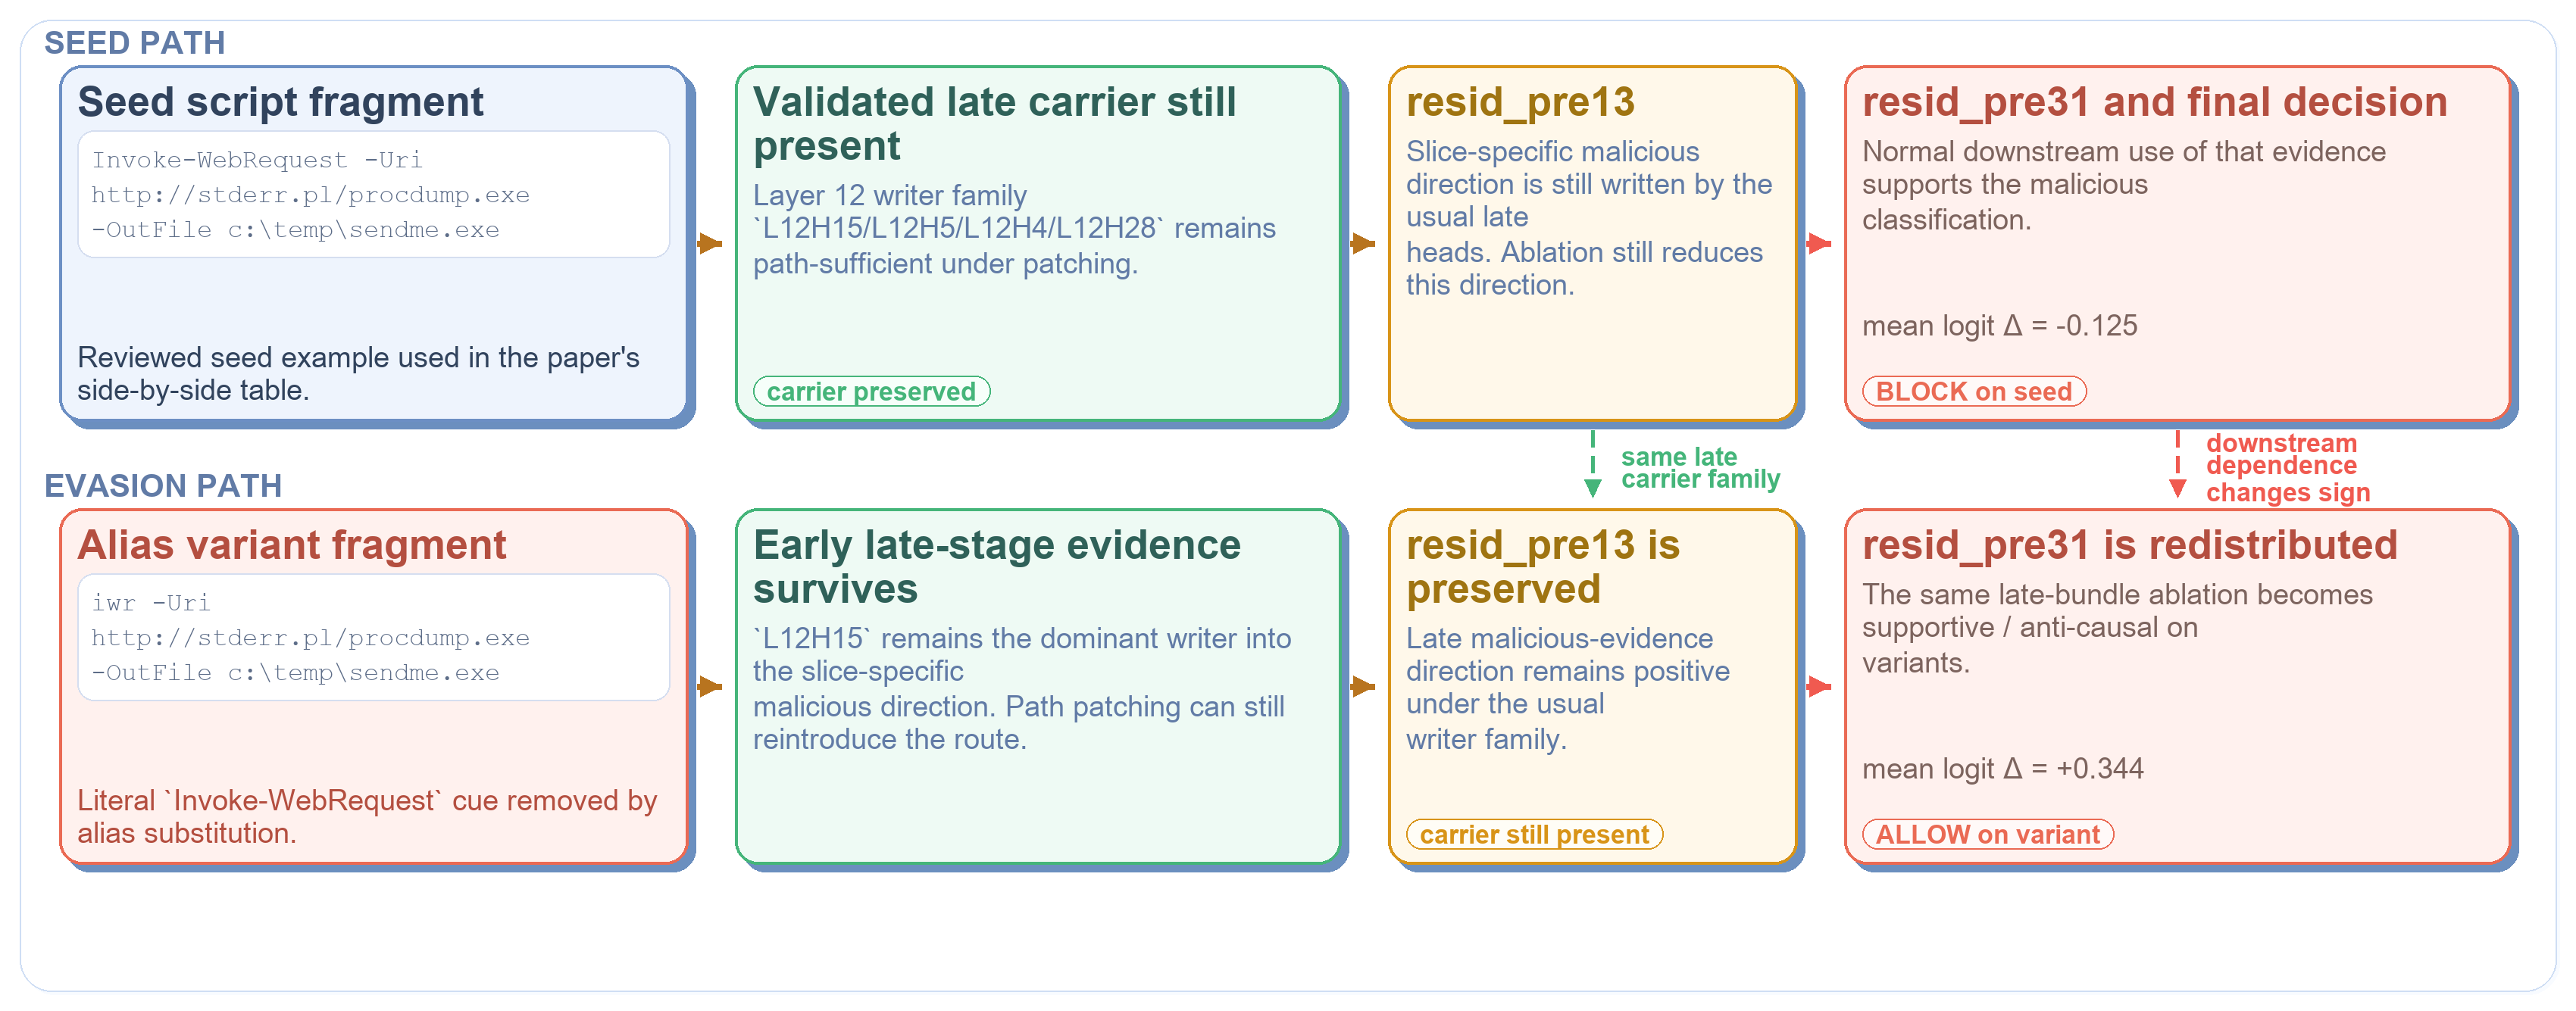
\includegraphics[width=0.92\linewidth]{artifacts/foundation_sec/figure_evasion_redistribution.png}
\caption{Conceptual summary of the strongest current successful-evasion interpretation. Under \texttt{invoke\_webrequest\_alias}, the late malicious-evidence bundle is still present, but competing computation before the Layer 13 boundary reverses how that evidence affects later computation, indicating signal reversal rather than simple route deletion.}
\label{fig:evasion-summary}
\end{figure}

\subsection{Monitoring Fine-Tuning Drift}
The comparative and evasion results support a practical operational extension. Foundation-Sec inherits the underlying PowerShell classification route from Llama, but its failures after fine-tuning are not best explained as deletion of that inherited mechanism. Instead, the current evidence points to a narrower change in how later computation uses that inherited signal: the relevant malicious-evidence representation still appears at the causally important \texttt{resid\_pre13} site, while downstream computation can suppress, redirect, or invert its effect for particular semantic families. This makes \texttt{resid\_pre13} a useful monitoring anchor for family-level regression testing after security fine-tuning.

\paragraph{Linear probe at the circuit boundary.}
We fit a linear probe (Ridge regression, 5-fold cross-validation) from the \texttt{resid\_pre13} activation of each malicious script to the per-head contribution of the four core Layer-12 heads measured by the head trace experiment. The probe achieves cross-validated \(r = 0.80\)--\(0.87\) for \texttt{L12H4}, \texttt{L12H5}, \texttt{L12H15}, and \texttt{L12H28} (\(n = 206\), all \(p < 10^{-45}\)). These values confirm that each head's contribution to the contrastive direction is \emph{linearly} encoded in \texttt{resid\_pre13} — meaning the information is directly readable as a simple linear projection of the inherited representation, not just extractable by a more flexible model.

Operationally, this gives a cheap drift quantity: run one forward pass through Llama and one through Foundation-Sec on canonical clean inputs, apply the same learned linear projection to each model's \texttt{resid\_pre13} activations, and compare the projected head contribution by capability family. If Foundation-Sec has preserved the inherited representation for a family, the family mean should remain close to the Llama mean. If fine-tuning compresses, rotates, or inverts that family's representation at the circuit boundary, the projected contribution will diverge. Applied cross-model at the script level, the same probe predicts Foundation-Sec's causal circuit dependence (\texttt{delta\_logit\_diff} under top-5 L12 ablation) at \(r = 0.41\) (\(n = 293\), \(p < 10^{-12}\)). This is useful but also sets the ceiling: per-script prioritization is noisy, so the intended operational unit is a family-level red-teaming priority, where averaging over scripts stabilizes the signal.

\begin{figure}[!htbp]
\centering
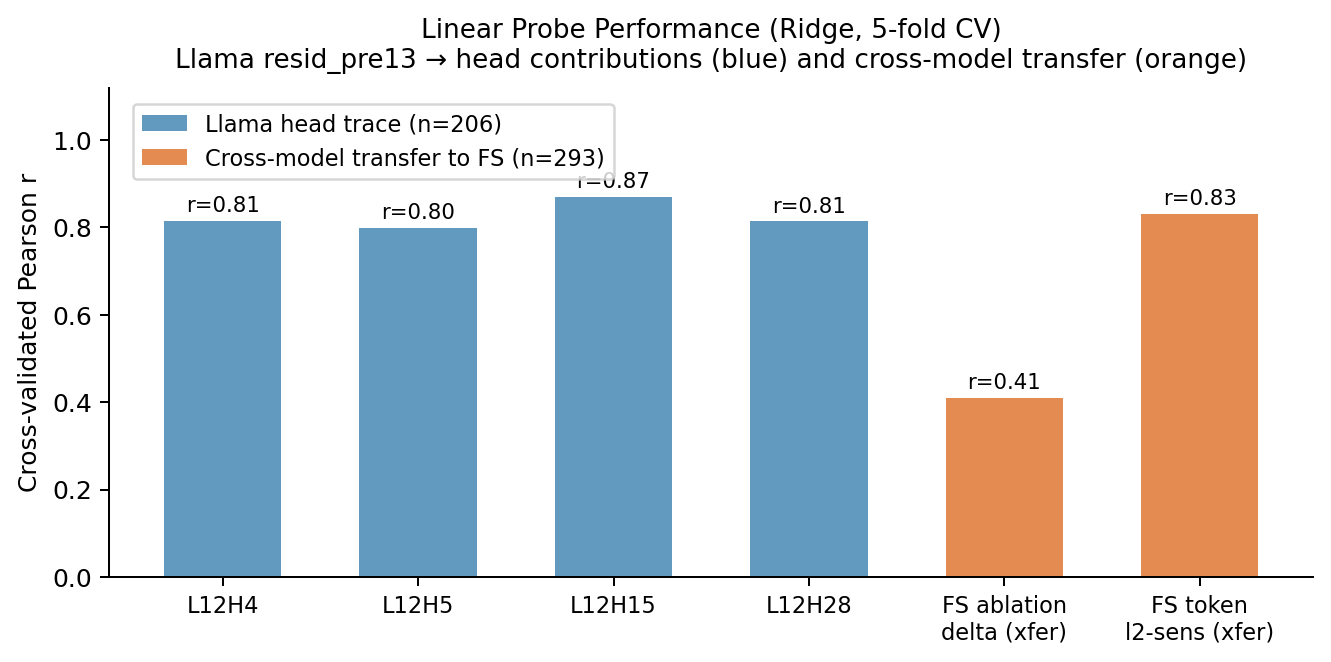
\includegraphics[width=0.92\linewidth]{artifacts/figure_linear_probe_r_values.png}
\caption{Cross-validated linear probe performance (Ridge regression, 5-fold CV). Blue bars show how well Llama's \texttt{resid\_pre13} activation predicts each Layer-12 head's contribution to the contrastive direction (\(r = 0.80\)--\(0.87\), \(n = 206\)). Orange bars show cross-model transfer: the same Llama activations predicting Foundation-Sec's circuit dependence under top-5 ablation (\(r = 0.41\)) and indicator-token L2 sensitivity (\(r = 0.83\)). The high within-model r values confirm each head's contribution is linearly encoded at the circuit boundary; the lower ablation-delta transfer (\(r = 0.41\)) reflects the ceiling imposed by the cross-model fine-tuning gap.}
\label{fig:probe-r-values}
\end{figure}

\begin{figure}[!htbp]
\centering
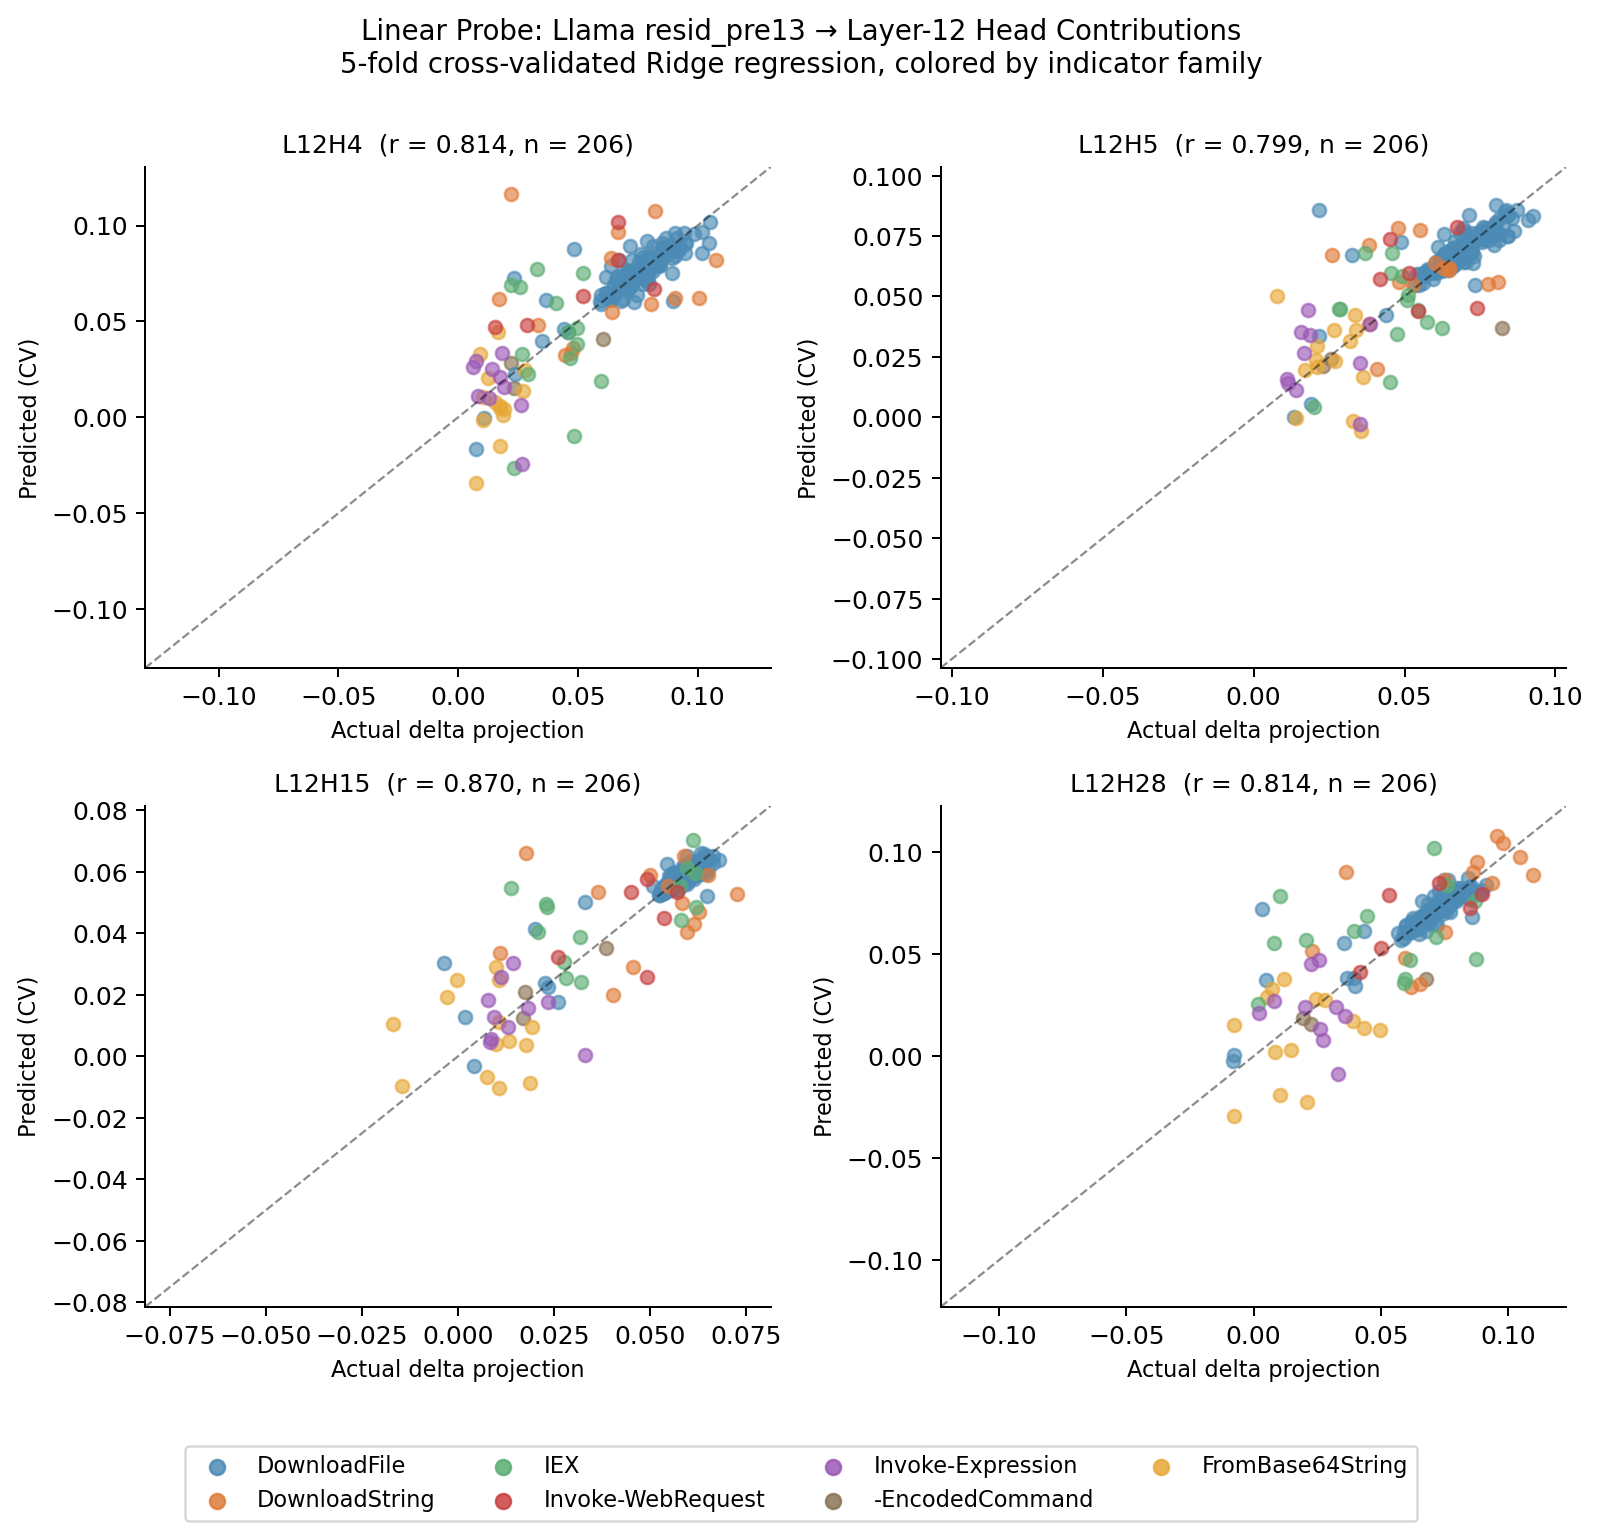
\includegraphics[width=0.92\linewidth]{artifacts/figure_probe_scatter_heads.png}
\caption{Scatter plots of predicted versus actual Layer-12 head contributions for each of the four core heads (\texttt{L12H4}, \texttt{L12H5}, \texttt{L12H15}, \texttt{L12H28}). Each point is one malicious script; the dashed diagonal is the identity line. Colors indicate indicator family. The tight alignment around the diagonal across all four panels confirms that the probe's \(r = 0.80\)--\(0.87\) performance is consistent and not driven by outliers or a single family.}
\label{fig:probe-scatter}
\end{figure}

The practical implication is not that the probe reliably ranks individual scripts by future evasion risk. Rather, the family-level average of the projected contribution under Llama versus Foundation-Sec reveals which capability families changed most in how strongly the inherited circuit is represented after fine-tuning. Those families are the natural first targets for adversarial variant generation.

\paragraph{Indicator-token sign inversion as an aliasing signal.}
The linear probe's cross-model transfer is strongest at the family level, where per-script noise averages out. But projection magnitude alone does not determine which changed families are specifically vulnerable to aliasing. A sharper signal comes from directly measuring how much each model's malicious classification confidence changes when the indicator command-name tokens are removed. For each malicious script, we replace the command-name token embeddings with an average neutral embedding (the mean across the model's full vocabulary) and measure the resulting change in the model's confidence score.

Most families in Foundation-Sec show the expected pattern: removing the indicator tokens reduces malicious confidence, consistent with those tokens acting as drivers of the malicious prediction. \texttt{Invoke-WebRequest} is the clear exception. Ablating its command-name tokens \emph{increases} average malicious confidence (\(+1.13\) mean logit-diff delta; 73.7\% of scripts show a positive delta), while Llama shows a strong negative delta (\(-1.60\)) for the same family. The divergence between the two models is most pronounced here: all other families stay within a narrow band, while \texttt{Invoke-WebRequest} is the only family with a large positive FS delta alongside a clearly negative Llama delta. Figure~\ref{fig:ablation-delta} shows the full family-level comparison.

\begin{figure}[!htbp]
\centering
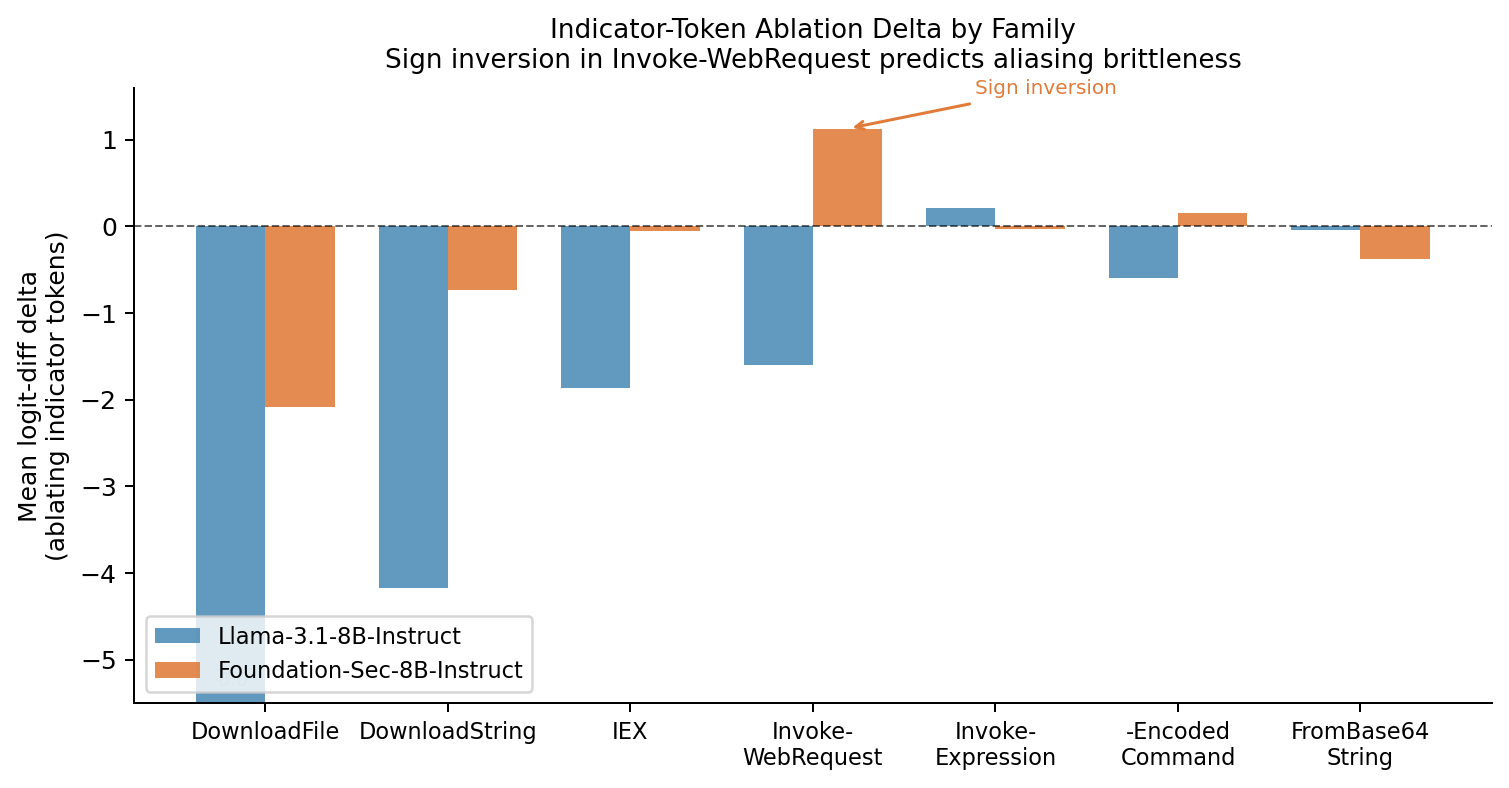
\includegraphics[width=0.92\linewidth]{artifacts/figure_ablation_delta_by_family.png}
\caption{Mean logit-diff delta when indicator tokens are mean-ablated, broken down by indicator family and model. A negative delta means removing the indicator tokens reduces malicious confidence (the token was acting as a driver of the malicious prediction). A positive delta means removing them increases malicious confidence (the token was acting as a suppressor). \texttt{Invoke-WebRequest} shows the clearest divergence: Foundation-Sec (orange) has a large positive delta (\(+1.13\)), while Llama (blue) shows a strong negative delta (\(-1.60\)). This divergence identifies \texttt{Invoke-WebRequest} as the family where the command-name token changed role between models — and where alias substitution (\texttt{iwr}) produces consistent classification failures. The DownloadFile Llama bar extends below the axis limit (value: \(-8.0\)); the y-axis is capped at \(-5.5\) to keep the smaller-delta families readable.}
\label{fig:ablation-delta}
\end{figure}

The mechanistic interpretation is that fine-tuning appears to have led Foundation-Sec to classify \texttt{Invoke-WebRequest} scripts through URL patterns, payload structure, and command arguments rather than through the command-name token itself. The evidence separates two effects. On canonical inputs, mean-ablating the full command-name token increases malicious confidence, so the token itself behaves like a suppressor. On the successful \texttt{iwr} variants, however, the validated late bundle still appears while later computation changes the downstream use of that evidence, indicating that the alias transformation also disrupts or reroutes the command-anchored payload-context signal. The miss therefore does not follow from suppressor removal alone; it follows from suppressor removal plus loss or inversion of the stronger contextual evidence path, with the latter dominating in the accepted variants tested here.

The linear probe also quantifies how much a script's internal representation shifts when its indicator tokens are removed: this shift is linearly predictable from the base-model activation at \(r = 0.83\) (\(n = 293\), \(p < 10^{-75}\)), confirming that token dependence is a stable, readable property of the inherited representation. The direction of that dependence — whether removing the tokens increases or decreases malicious confidence — is the operative aliasing signal. A family where the fine-tuned model's ablation delta flips sign relative to the base model should be prioritized for token-substitution attacks, and this flip is detectable on canonical clean inputs without generating any evasion variants in advance.

Operationally, this motivates a two-stage family-level monitoring recipe:
\begin{enumerate}[leftmargin=1.5em,itemsep=0.2em,topsep=0.2em,parsep=0pt]
  \item \textbf{Fit a drift detector:} using the base model and a set of canonical malicious scripts, train a linear probe that predicts how strongly each key attention head contributes to the classification decision from the model's internal state at the circuit boundary.
  \item \textbf{Compare base and fine-tuned models:} run both models on the same canonical inputs, apply the probe to each, and compare the results by command family. Families where the fine-tuned model's score diverges strongly from the base model have drifted most in how they use the inherited circuit.
  \item \textbf{Run the sign test:} for each family, remove the command-name tokens in both models (replacing them with a neutral average embedding) and measure whether confidence goes up or down. A family where the fine-tuned model's confidence \emph{increases} when the command name is removed — but the base model's confidence \emph{decreases} — has undergone a role reversal and is an alias attack surface.
  \item \textbf{Prioritize red-teaming:} generate alias and command-reconstruction variants for the flagged families and test them against the fine-tuned model.
\end{enumerate}

Both steps use only canonical clean inputs — no evasion variants need to be generated in advance, and no retraining is required. In this study, the sign test correctly identifies \texttt{Invoke-WebRequest} as the red-teaming priority before any alias variants are tested.

\section{Limitations}
The main limitation is scope. The mechanistic and evasion claims are based on one fine-tuned model, its Llama base model, and one PowerShell classification setting. The cross-model comparison is therefore a strong control for this model pair, but it does not by itself establish that all security fine-tunes will develop the same brittleness. The evasion benchmark also contains small positive slices: the strongest failures are \(4/4\) accepted \texttt{Invoke-WebRequest} alias variants and \(4/4\) accepted \texttt{Invoke-Expression} format-string variants. These are important counterexamples, but they should be treated as red-teaming signals rather than population-level evasion-rate estimates until replicated with larger per-family coverage.

The matched cohort is filtered to examples that both members of each pair handle correctly at baseline, which is useful for causal interpretation but narrows the evaluated distribution. The activation-space monitoring result is also strongest at the family level: cross-model transfer to Foundation-Sec ablation dependence reaches \(r = 0.41\), so individual-script prioritization should be treated as noisy rather than deployment-ready. The analysis also does not fully identify which specific feed-forward components reverse the classification signal in the successful evasion cases — we can observe that the reversal happens near Layer 13, but have not localized exactly which component is responsible. Finally, the observed brittleness is consistent with command-name correlations in the fine-tuning data, but we do not directly measure the training corpus to confirm this specific cause.

\section{Future Work}
Next steps for this line of work can include extending the validation cohort to cover additional indicator families beyond the seven reported here and to deeper per-family pair counts, so that the current 293-pair result can be stress-tested with a more independent validation design. On the robustness side, the evasion benchmark can expand along two fronts: deeper coverage inside the already active \texttt{keyword\_hiding}, \texttt{string\_construction}, and \texttt{execution\_indirection} families, and concrete tests for two currently theoretical families. \texttt{network\_object\_indirection} would hide direct networking surfaces behind equivalent object-construction, method-dispatch, or reflection patterns. \texttt{staged\_payload\_flow} would preserve the same malicious behavior while splitting retrieval, decoding, allocation, and execution across intermediate variables or helper functions.

On the mechanistic side, the main open question is which specific feed-forward components reverse the classification signal in the successful evasion cases. The current evidence shows the reversal happens near the Layer 13 boundary but does not yet identify the responsible components precisely. Future work should localize these, and compare how Foundation-Sec handles full-form command names versus aliases at that site — this would directly explain why the suppressor effect is specific to \texttt{Invoke-WebRequest} and \texttt{Invoke-Expression} rather than other families. Most importantly, the detection workflow — linear probe drift screen plus indicator-token sign test — should be validated on additional security fine-tunes and command families to assess how broadly the sign-flip pattern generalizes as a red-teaming prioritization signal.

\section{Conclusion}
Security fine-tuning improves LLM classification on the inputs it was trained to handle — and, as this study shows, can simultaneously introduce alias vulnerabilities that standard evaluation is not designed to detect. A model trained on a corpus where specific command names are correlated with maliciousness will score well on held-out test data while silently failing on scripts that use common short-form equivalents. This is not a model quality problem in the conventional sense; it is a gap between what evaluation measures and what adversaries can exploit.

We demonstrate this concretely for Foundation-Sec-8B-Instruct using mechanistic interpretability tools applied to a natural base/fine-tuned model pair. Causal interventions on a 293-pair matched cohort localize the classification circuit to a Layer-12 attention bundle inherited from Llama — fine-tuning concentrated and semantically specialized this existing structure rather than building a new one. That specialization is what creates the vulnerability: Foundation-Sec learned to classify \texttt{Invoke-WebRequest} scripts through payload context rather than the command name itself, making the full command name a suppressor rather than a driver. The evasion benchmark confirms the consequence — consistent misses on \texttt{iwr} substitution that Llama, with its more diffuse inherited representation, does not share. To our knowledge this is among the first mechanistic circuit analyses in a cybersecurity LLM context, combining causal validation, cross-model comparison, and a matched seed/variant evasion benchmark \citep{choi2020malicious,garciacarrasco2024detecting}.

The practical output is a two-step pre-deployment workflow that any team fine-tuning an LLM for security classification can apply. First, a linear probe from base-model activations at the classification boundary (\(r = 0.80\)--\(0.87\) per head) identifies which capability families drifted most in how strongly the inherited circuit engages after fine-tuning. Second, an indicator-token sign test — comparing how each model's confidence responds to command-name ablation on canonical clean scripts — flags the specific families where the token role flipped from driver to suppressor. Both steps require only forward passes on canonical inputs; no evasion variants need to be generated in advance. In this study the sign test correctly identifies \texttt{Invoke-WebRequest} as the red-teaming priority before any alias variants are tested. The method is not a per-script evasion predictor, but it provides a principled family-level prioritization signal that standard accuracy evaluation does not.

\bibliographystyle{plainnat}
\IfFileExists{references.bib}{\bibliography{references}}{\bibliography{../references}}

\end{document}
